This chapter presents methods used to evaluate the system; results collected evaluating the system and a discussion around the system. 

\section{Methods}
\subsection{User Survey}

The system is measured by doing user surveys on the end users. In our user survey we have coaches’ and others with many years of experience in soccer rating how much they agree with a statement on a Likert-scale. The statements compare the system against other systems in use at Alfheim today. For other’s we evaluate the system as a stand alone analytic system. The Likert-scale chosen is a 5 point scale from \textit{strongly disagree} to \textit{strongly agree}.\footnote{http://www.simplypsychology.org/likert-scale.html}. In short it will let each individual to note how much they disagree or agree with a particular statement.

We will also let assessors comment about the usability or other things of the system that will be taken into the evaluation. 

\subsection{UI Performance}

Measuring \ac{UI} Performance is way of measuring usability of the system. These two are directly linked up to each other \cite{satisfaction}. A slow system and unresponsive system decrease satisfaction and usability for the end-user. Foundings in \cite{nielsen} indicated that a response time of longer than 1000ms would decrease the satisfaction of the user. The thought-flow of the user will not be interrupted and therefor one can argue that the \ac{UI} it's fast enough. We will use this threshold to evaluate our UI performance in the system. 

To measure the UI Performance we use Google Chrome DevTools\footnote{https://developers.google.com/chrome-developer-tools/}. A web page is only fully loaded when all requests have been fully received. In our \ac{SPA} new requests will be spawned after the \ac{DOM} is loaded. Therefor, we run performance tests for both fully reload of the page, when the DOM is ready and when the users navigates in already rendered page, which will be the most typical way for the user to navigate to different pages.

\subsection{Compatibility}

In the requirement specification we stated that going for a web page would ensure compatibility and accessibility. Every device now has a web browser and therefor the page can be reached from anywhere as long as you have an Internet connection. 

To test this we use PowerMapper\footnote{ http://try.powermapper.com/demo/sortsite } website testing and site mapping tool. This test checks a wide range of things like browser support, dead links and accessibility. We use it for compatibility testing for web browsers.

\section{Experiments and Results}

In the tests \ac{TIL} and external experts in soccer have been used to evaluate the system. In the tests we are looking to see if we have achieved our goals listed in the requirements. To recapture the main goals; we wanted to create a system that difference it from the existing systems teams and at the same time provide information that can be used for opponent soccer analytic. We specifically wanted to identify key players.

\subsection{Database size}
In figure \ref{fig:dbsize} the size of the different indexes in the database is listed. Match related data is stored in the match, attack and pass index. The total size of those 3 indexes is 379.5kb and with a total of 12 matches in the database. This means that an average match stored takes around 31.6kb of storage.

\begin{figure}[ht!]
\centering
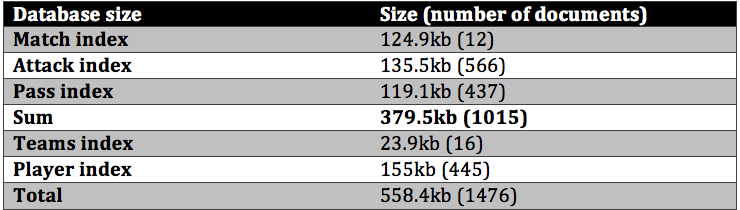
\includegraphics[width=1\textwidth]{images/evaluation/dbsize}
\caption{Table with the size of each index and the total size of all indexes}
\label{fig:dbsize}
\end{figure}

\subsection{Test data}

In the evaluation the database had been populated with data from \ac{TIL} and Str{\o}msgodset matches. Only attacks from these two teams have been used to answer the user servey. A total of 34 attacks have been captured for Str{\o}msgodset over 5 matches. For \ac{TIL} a total of 42 attacks have been captured over 9 matches. Figure \ref{fig:matches_regged} lists all matches. Some matches include data from other teams than \ac{TIL} and Str{\o}msgodset. They have not been taken into consideration in the evaluating process.

\begin{figure}[ht!]
\centering
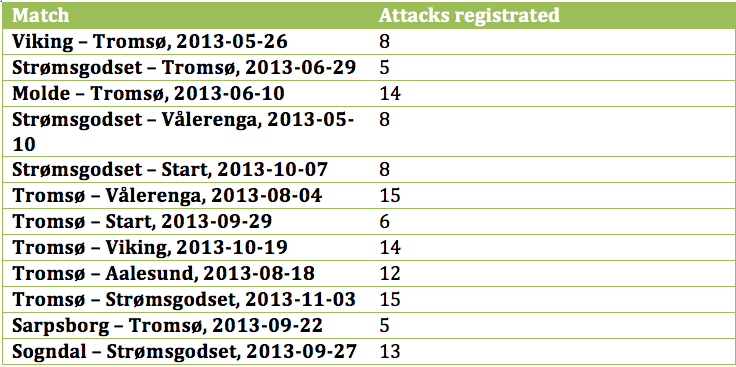
\includegraphics[width=1\textwidth]{images/evaluation/matched_regged.png}
\caption{Matches that have been captured and persisted into the database}
\label{fig:matches_regged}
\end{figure}

\subsection{SAT as a tool for opponent analytic}
% SAT gives you valuable information about opponents that the current systems you use today don’t provide

In this user servey the assessors where asked how SAT is as a complementary opponent analytic tool. In the requirement process we specified that the system should to be a complementing tool and not a direct replacement of the systems in use. The results shown in figure \ref{fig:user_servery1} shows that most of the assessors values the information the system provides. 

\begin{figure}[ht!]
\centering
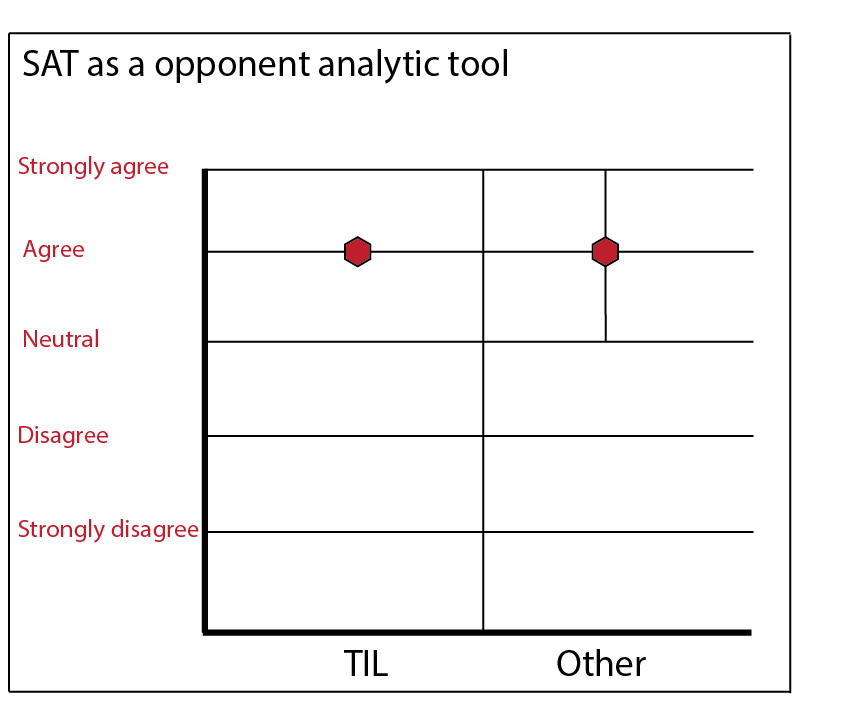
\includegraphics[width=1\textwidth]{images/evaluation/user_servery1}
\caption{SAT as a tool for opponent analytic. Experts answers varying from neutral to strongly agree.}
\label{fig:user_servery1}
\end{figure}

Assessors not in the \ac{TIL} system do not necessarily use or have experience with an existing tool for opponent analytic. Therefor the statement was re-phrased. The assessors were asked how SAT is as an opponent analytic tool, a stand-alone product. The results listed at the right side in figure \ref{fig:user_servey1} shows that the majority of assessors was satisfied we the system with answers varying from neutral to strongly agree.

From these results we can conclude that the assessors view the Soccer Analytic Tool as a good system for providing information about soccer opponents. The assessors would have the system rather not having it. Assessors not from \ac{TIL} has various experience in using analytic tools. SAT was developed with the knowledge of the systems that was in use at Alfheim today. We speculate that this is the reason the system is not as appealing for people not in the \ac{TIL} system. It is unclear what tools others is using or has experience with.

\subsection{SAT as a tool for identifying key players}

In this user servey the assessors where asked how SAT is as a tool for identifying key players in a soccer team. This was one of the main goals of the system. The results of the user servey is shown in figure \ref{fig:user_servery2}. 

\begin{figure}[ht!]
\centering
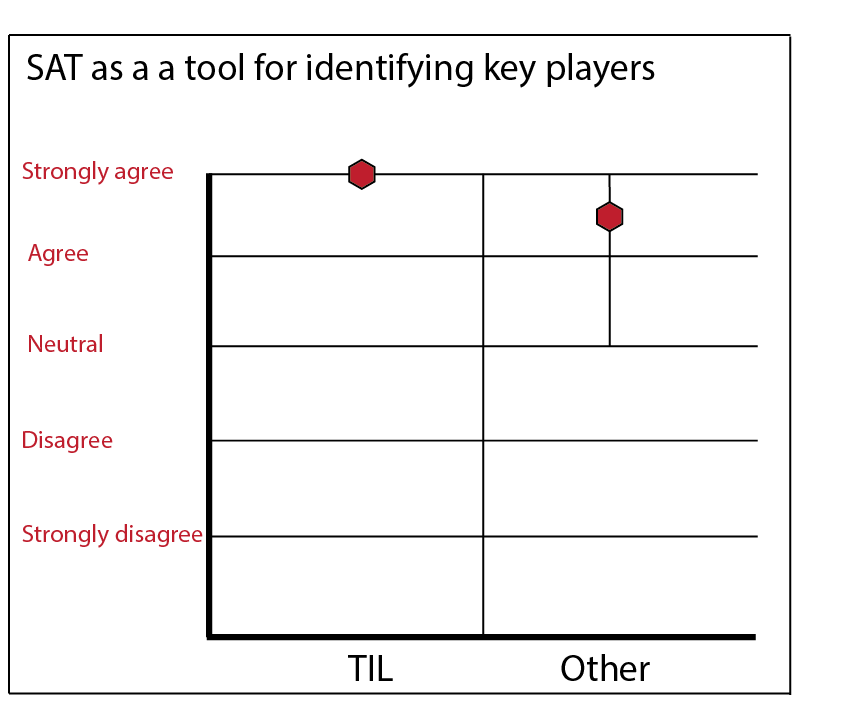
\includegraphics[width=1\textwidth]{images/evaluation/user_servery2}
\caption{SAT as a tool for identifying key players. Experts answers varying from neutral to strongly agree.}
\label{fig:user_servery2}
\end{figure}

We can see from the results of the user servey that the assessors agrees strongly that the system lets you identify key players in the opponent team. Assessor’s answers varying from neutral to strongly agree.

\subsection{User servey comments}
Assessors came with comments including to answering the user servey. These comments are summarized in figure \ref{fig:comments}.

\begin{figure}[ht!]
\centering
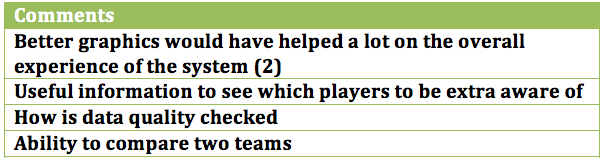
\includegraphics[width=1\textwidth]{images/evaluation/comments}
\caption{User servey comments}
\label{fig:comments}
\end{figure}


\subsection{UI-performance}
UI performance was measured by testing the most content rich web page the team analytic page for \ac{TIL}. All the response times were measured by doing 20 samples. Tests where run at localhost with server and database running on the same machine, meaning that a further increase in time would likely be seen if the system was in production. Total size for all requests was 1.6 MB. Figure \ref{fig:uiperform} lists the results.

\begin{figure}[ht!]
\centering
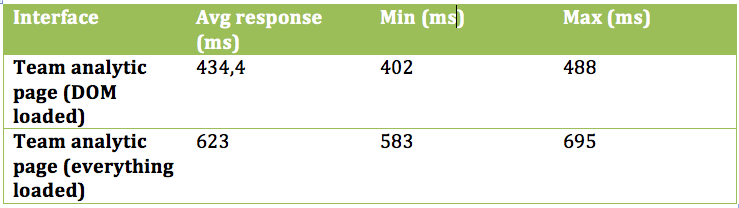
\includegraphics[width=1\textwidth]{images/evaluation/uipeform}
\caption{UI Performance test results. }
\label{fig:uiperform}
\end{figure}

Two tests were run to see the difference of a \ac{DOM} load and a fully page load (all requests to the back-end done). The difference between the two is that in the latter we also add the time for the requests for team statistics as these requests are run when the JavaScript code is executed. The user will see that the page is loaded but is missing some content because of the team statistics requests.

The results show that we are well below the 1000ms threshold in both tests Nielsen \cite{nielsen} suggested. The maximum delay was 695 ms over the 20 samples for complete page load and 488 ms for \ac{DOM} load. Requests for team statistics took in average 188.6 ms to complete. This includes 3 requests to the back-end API:
\begin{itemize}
\item \emph{/team/Troms{\o}/finalthird}: Passes into final third of the pitch.
\item \emph{/teams/Troms{\o}}: Team statistics.
\item \emph{/players/Troms{\o}}: Fetching all players.
\end{itemize}


\subsection{Compatibility}

Figure \ref{fig:compa} shows the result after running the page in different web browsers with the PowerMapper tool. The results show that the web page works in most browsers except from some issues in older Internet Explorer versions. We can conclude that the page has good compatibility with different web browsers making in accessible on many platforms.

\begin{figure}[ht!]
\centering
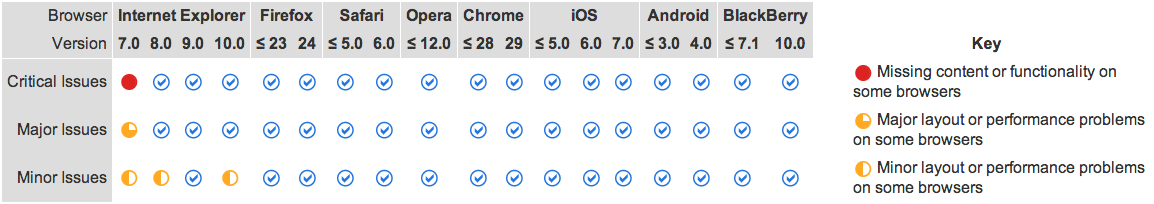
\includegraphics[width=1\textwidth]{images/evaluation/compa}
\caption{Compatibility test by running the web page in different browsers. Screenshot from powermapper.com free trial version}
\label{fig:compa}
\end{figure}

\section{Discussion}
\subsection{Input}

Perhaps the biggest limitation of the system is that it requires manual work to be functional. The system requires a lot of manually work to be operational as an opponent analytic tool. Up to one hour is the normal time spent capturing all data for a match with the current capture interface. On average, teams across the top four top leagues (La Liga, Premier League, Serie A and Bundesliga) took about 13 shots per match, measured in the 2010/11 season \cite{soccerbynumbers}. This means you will have possible have 26 attacks to capture for each match. 

In section \ref{sec:capprocess} it is mentioned that you have to store the players by their ID. IDs are only found in the database. Instead of this a player selector interface could have been developed letting you just click on an image of the player involved and the ID will be automatic inserted in. We suggest you can save up to 20 minutes by having this feature added.

\subsection{Accuracy}

There is minimal quality checking of the input data except from the match view page that lists every attack captured, meant for external operators to verify the data. Other than that you have to trust the operator that is capturing match data. The input is to some degree subjective for some data like identifying breakthroughs. In some cases one operator may say that it was a breakthrough and another operator does not agree. This may not be the biggest problem if you set some rules to follow for the operators. Identifying the zone for an event can also be a bit tricky. Especially, in soccer stadiums that have a low camera angel when being filmed. 

In our test data an average match is around 31.6kb size large, but we only capture attacks from one team. However, it is nothing in comparison with ZXY where a match is around 500-700mb. A more fear comparison would be against Opta’s data size for a match, as they are more in the same genre as our system, using only manual input. As previously mentioned, they capture every pass in the game meaning that they most likely store more data per match than our system. 

\subsection{Domain model}
The domain model has been dedicated a lot of time to in the process of defining and building the system. It was crucial to have a domain model that reflected what type of opponent analytic information the system should give the end-user. What is enough data? Having a larger domain model would increase time spent in the process of capturing data. 

A thing that could have been changed to get more precise analytic information is how breakthroughs are represented in the database. The current solutions store each type of breakthrough as text saying where on the pitch the breakthrough came from. Rather than this, we could have taken advantage of the already defined dividing of the pitch. This would have given use more precise data to present to the end-user.

\subsection{UI Performance}

A thing to take into consideration is the amount of matches in the database under the tests. A system in production would contain a lot more matches and would increase the response time. 

In a \ac{SPA} you don't necessary get all the files at once, but when you need them. On render, the web browser will first get the root \ac{HTML} document and then start requesting all other files that is referenced in the document, like \ac{CSS} and JavaScript files. Bundling all JavaScript files can to one file would save a lot of network traffic. Doing a complete reload of the team analytic page Google Developer Tools reports that total 55 requests is done to the back-end, fetching various files and requests to the REST API.

\subsection{Usability}

Several assessors noted that improving the graphical components would increase the overall experience of the system and make the system easier to use. This has not been one of the main focuses during the development of the system. However, from the results of the user servers the system must be to some degree usable in the way of the assessors find the information useful. 







